\documentclass[11pt]{article}
\usepackage[margin=2.2cm]{geometry}
\usepackage[T1]{fontenc}
\usepackage{amsmath,amssymb,booktabs,graphicx,xcolor,enumitem,tikz,caption}
\usepackage[section]{placeins}
\usepackage{hyperref}
\usetikzlibrary{positioning,arrows.meta}
\setlist{itemsep=2pt,topsep=3pt}
\hypersetup{colorlinks=true,linkcolor=blue!50!black,urlcolor=blue!50!black}
\captionsetup{font=small,labelfont=bf}

\definecolor{trace}{HTML}{2A78D6}
\definecolor{image}{HTML}{C9551F}
\definecolor{model}{HTML}{13865D}
\definecolor{ink2}{HTML}{4A5462}
\tikzset{
  box/.style={draw=#1,fill=#1!8,rounded corners=3pt,align=center,font=\footnotesize,minimum height=1cm,text width=1.9cm,line width=0.7pt},
  box/.default=ink2,
  arr/.style={-{Stealth[length=2.2mm]},line width=0.8pt,color=ink2},
}

\title{Level 1: predicting skipper-CCD noise from short readout traces\\[3pt]
\large Pipeline, models, first real data and what carries over to other CCDs}
\author{ccd\_opt\_ml}
\date{PA03, board 101 (acm101); 43 packets of 2026-11-02/03; analyses up to 2026-11-04}

\begin{document}
\maketitle

\section*{Summary}
\begin{itemize}
\item \textbf{Goal.} Find good CCD settings without taking a 5--10 minute image at every try, by predicting the image's
  read noise $\sigma_e$, dark charge $\lambda$ and gain $g$ from a readout trace taken in seconds.
\item \textbf{$\sigma_e$ works and transfers.} A physics-structured model reads $\sigma_e$ off the trace's white noise:
  6--7\,\% error on the held-out session C, about 14\,\% on an amplifier the model never saw.
\item \textbf{$\lambda$ and the gain} looked excellent on board 101 (5.3\,\% and 0.9\,\% on session C), but mostly
  because the reference trace identifies the amplifier. On a new amplifier no model beats the average until its level is
  measured once (one image or one level-1 strip); after that the gain is at about 1\,\% and the $\lambda$ models still
  beat the average.
\item \textbf{Inputs.} Leaving out the noisy channel (101 ch2 = EXT3), the amplifier-fingerprint features and the
  settings makes nothing worse and lets $\lambda$ beat the average on a new amplifier for the first time
  (39.7\,\% against 51.5\,\%). The learning curve is still falling at 32 packets: more packets help.
\item \textbf{Next.} The v2 night (76 packets, joint design, level-1 strips in every packet, settings changed on every
  working board), then a test on a second CCD.
\end{itemize}

% ======================================================================================================
\section{The goal and the physics}

An image (16 rows $\times$ 1000 columns $\times$ 500 skips) takes 5--10 minutes; run\_WADERs fits it and gives the
truth. A trace ($2\times5$ pixels $\times$ 500 skips, every raw ADC sample kept) takes about 2 seconds. Level 1 asks
whether the trace already tells us what the image will show. Level 2 would suggest settings from the predictions,
level 3 would run the scans itself.

A skipper CCD moves each pixel's charge back and forth under the sense node and measures it $N$ times without
destroying it. Averaging $N$ skips lowers the read noise until slow noise sets a floor:
\begin{equation}
\sigma_{\rm ADU}^2(N)=\frac{\sigma_1^2}{N}+\sigma_{\rm floor}^2,\qquad \sigma_e=\frac{\sigma_{\rm ADU}}{g}.
\end{equation}
On board 101 $\sigma_1\approx5.6$ ADU, so with $N=500$ the white part is $0.25$ ADU, about $0.19\,e^-$ at $g=1.3$.
The three targets are the image's $\sigma_e$ (0.15--0.19 $e^-$), $\lambda$ (mean charge per pixel: dark current
collected while rows wait, plus clock-induced charge, CIC) and $g$ (1.26--1.34 ADU/$e^-$).

\begin{figure}[h]
\centering
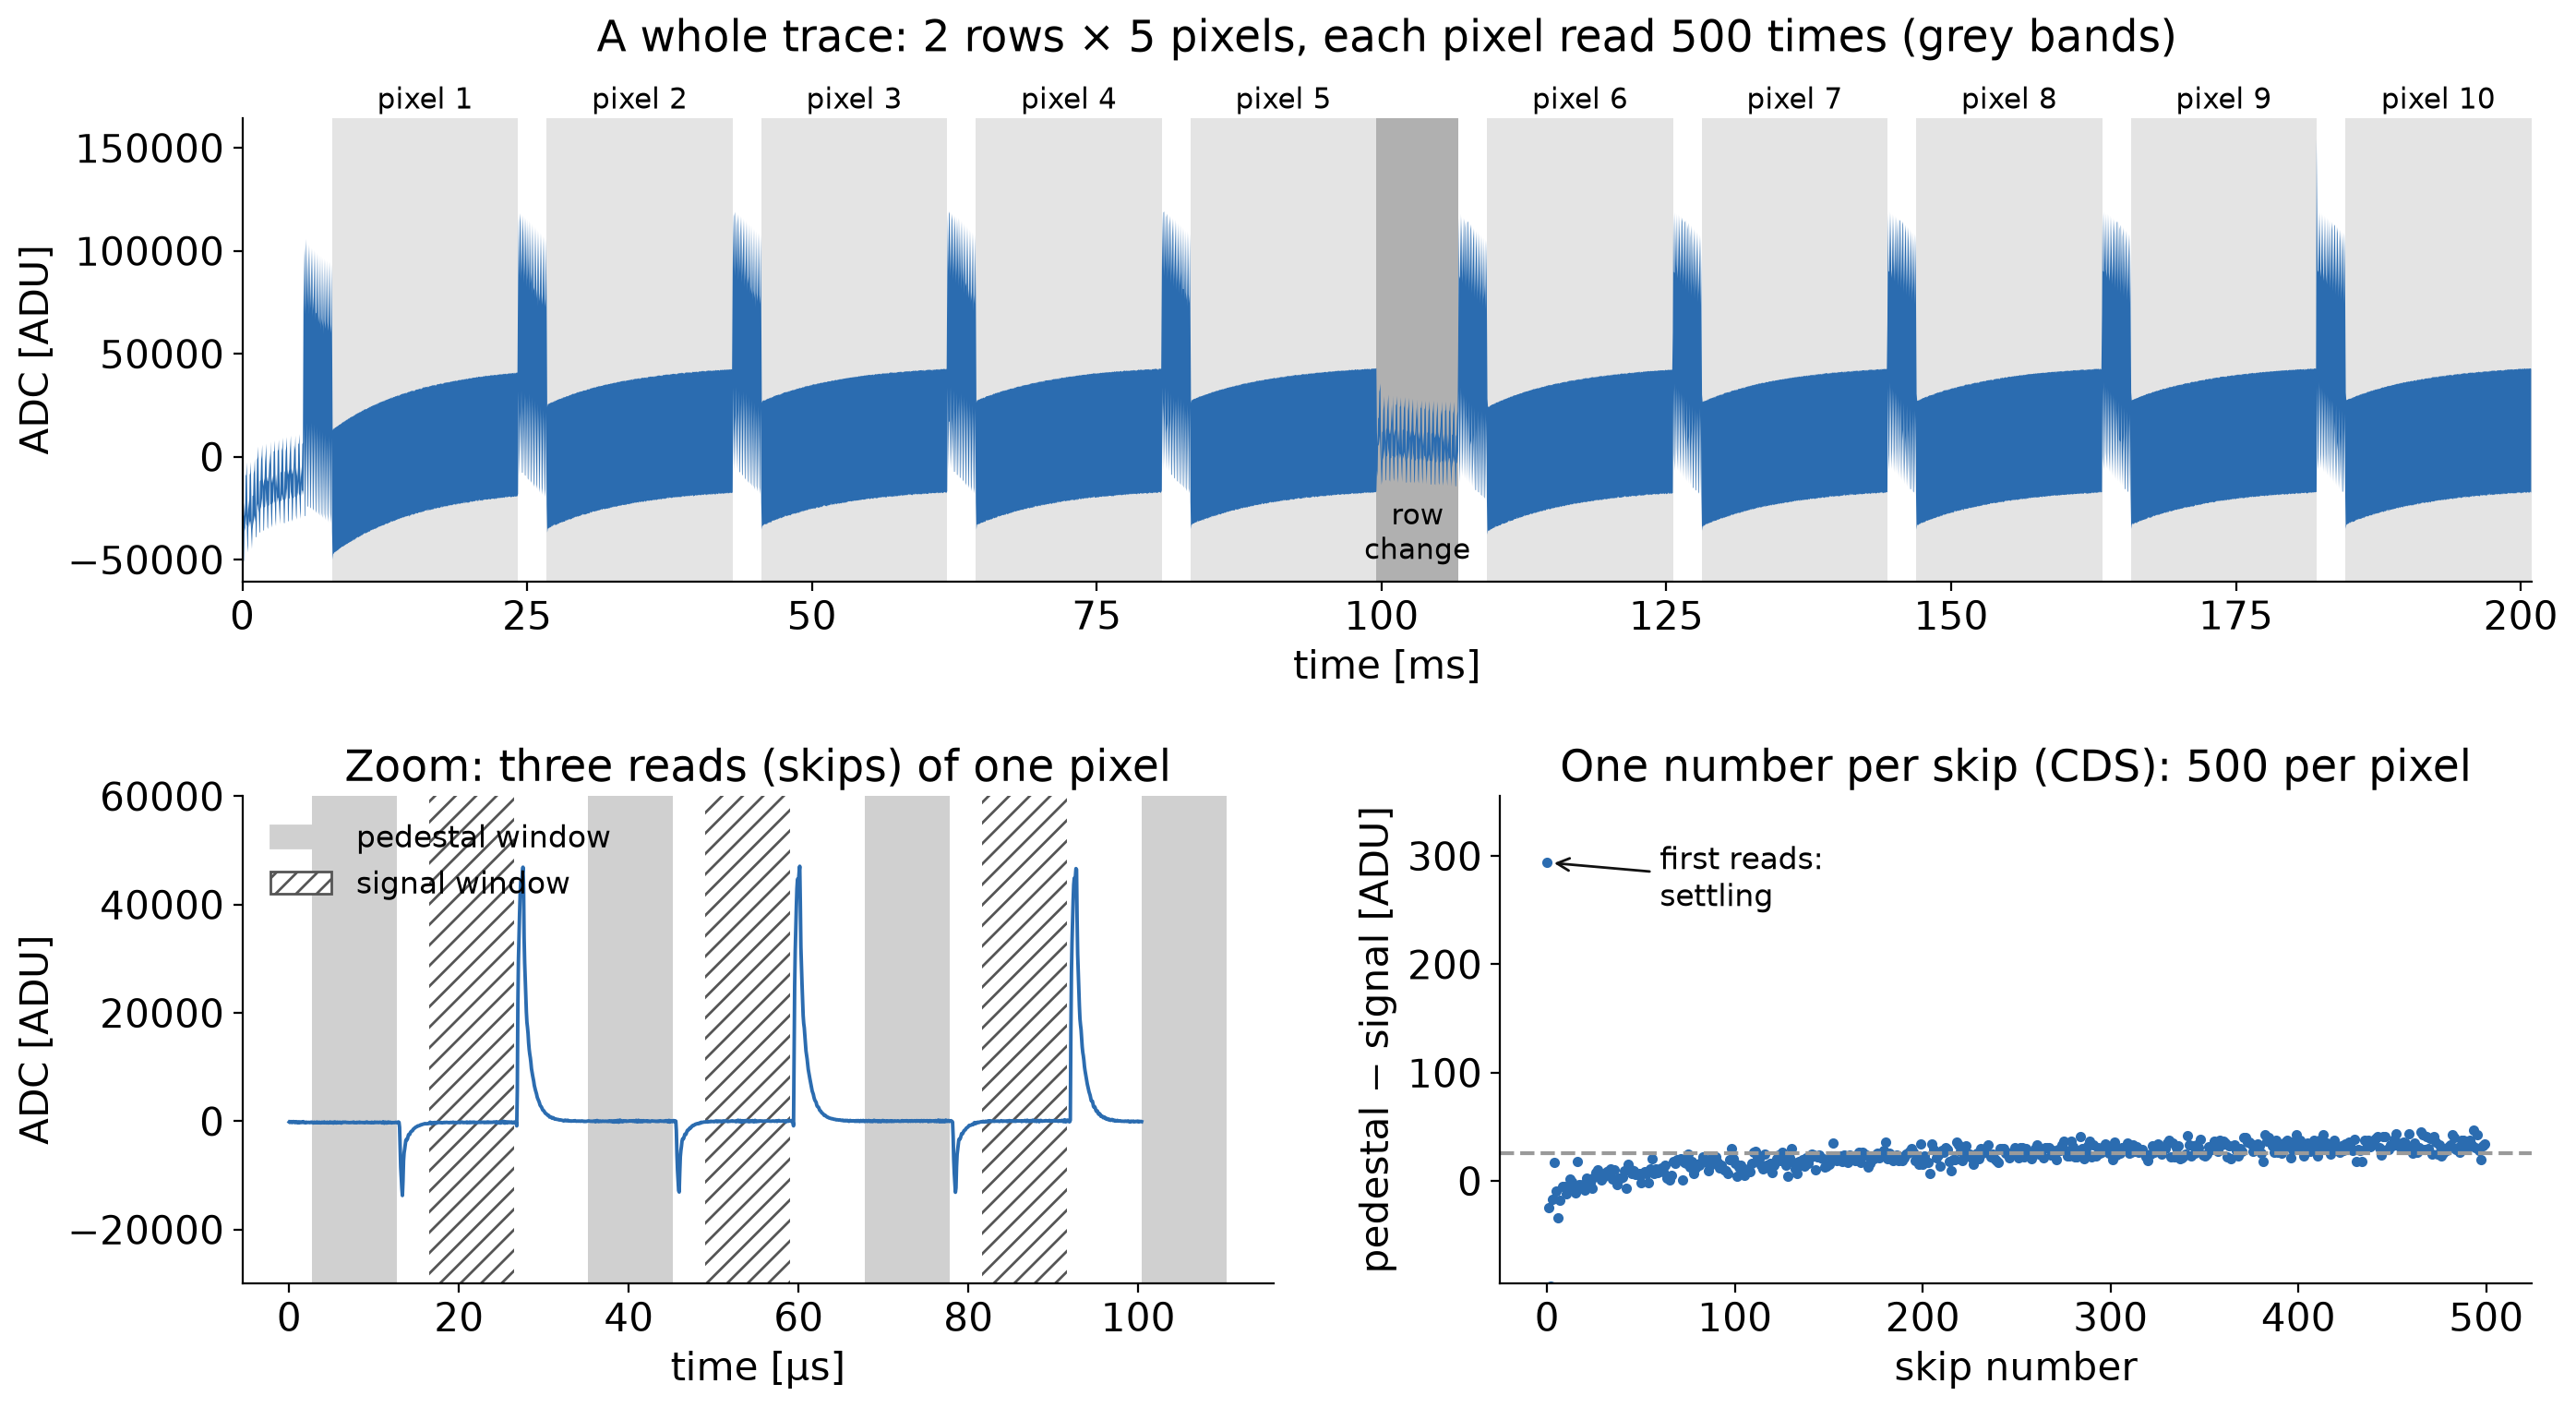
\includegraphics[width=0.75\textwidth]{figures/reuse_t_trace_anatomy.png}
\caption{A trace: 10 pixels, each read 500 times. Each skip has a pedestal window and a signal window; their
difference (CDS) is one number per skip. The image keeps only pixel averages; the trace keeps the waveform.}
\end{figure}

Each trace is turned into 141 scalar features and 16 curves of 256 points (src/trace\_features.py): noise (CDS
$\sigma$, white noise per skip, Allan and Hadamard deviations, 1/f corner, band powers), skip (first-skip excess,
ringing, droop), edge (reset pulse and SW dip shape, jitter, recovery), slow, start and clock features, and curves
(Allan deviation, spectra, mean skip shape, start transient). The Allan curve is fitted as
$\sigma_A^2(n)=a^2/n+b^2$ with $a=\sigma_1$ and $b=\sigma_{\rm floor}$.

% ======================================================================================================
\section{From the DAQ to a training table}

\subsection{Packets}
\begin{center}
\resizebox{0.97\textwidth}{!}{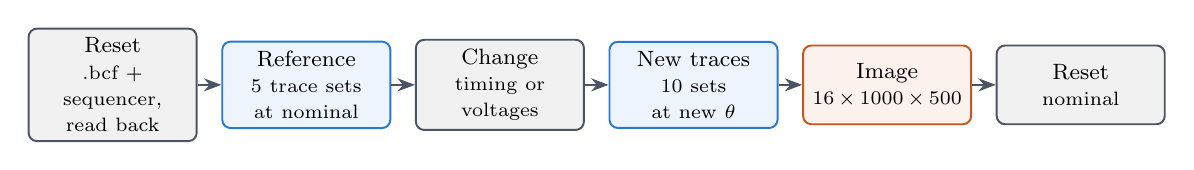
\begin{tikzpicture}[node distance=0.3cm]
\node[box] (a) {Reset\\\scriptsize .bcf + sequencer, read back};
\node[box=trace,right=of a] (b) {Reference\\\scriptsize 5 trace sets at nominal};
\node[box,right=of b] (c) {Change\\\scriptsize timing or voltages};
\node[box=trace,right=of c] (d) {New traces\\\scriptsize 10 sets at new $\theta$};
\node[box=image,right=of d] (e) {Image\\\scriptsize $16\times1000\times500$};
\node[box,right=of e] (f) {Reset\\\scriptsize nominal};
\foreach \x/\y in {a/b,b/c,c/d,d/e,e/f} \draw[arr] (\x)--(\y);
\end{tikzpicture}}
\end{center}
One packet gives four training rows (one per amplifier); the models are never told which amplifier a row is. The night
of 2026-11-02 had 43 packets: session A (14, timing changed one at a time), B (18, voltages one at a time) and C (11,
several knobs at once, the held-out test). Only board 101's settings were changed. Five nominal packets measure how
well the labels repeat.

\textbf{Safety.} \texttt{nominal()} restores both the voltages (.bcf) and the sequencer (clock timing) and reads them
back (biases within 0.3\,V, offsets and rails within 0.05\,V, every delay and the sequencer name); a mismatch stops the
packet. Traces are checked on the spot and damaged ones retaken (v2). All 43 packets started at nominal; 2370 of 2580
board-101 traces were usable.

\subsection{Processing}
\begin{center}
\resizebox{0.92\textwidth}{!}{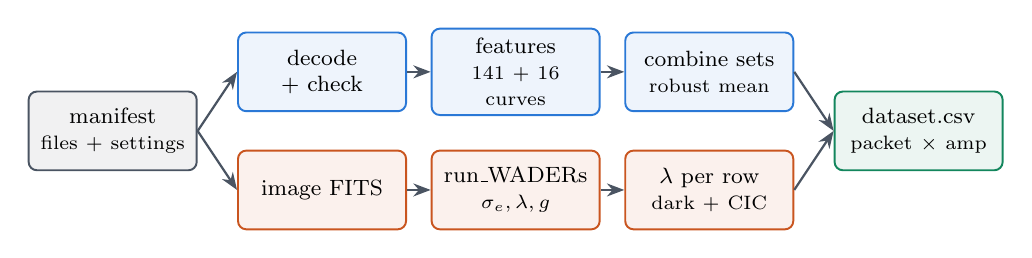
\begin{tikzpicture}[node distance=0.3cm and 0.3cm]
\node[box] (m) {manifest\\\scriptsize files + settings};
\node[box=trace,right=0.5cm of m,yshift=0.75cm] (t1) {decode + check};
\node[box=trace,right=of t1] (t2) {features\\\scriptsize 141 + 16 curves};
\node[box=trace,right=of t2] (t3) {combine sets\\\scriptsize robust mean};
\node[box=image,right=0.5cm of m,yshift=-0.75cm] (i1) {image FITS};
\node[box=image,right=of i1] (i2) {run\_WADERs\\\scriptsize $\sigma_e,\lambda,g$};
\node[box=image,right=of i2] (i3) {$\lambda$ per row\\\scriptsize dark + CIC};
\node[box=model,right=0.5cm of t3,yshift=-0.75cm] (ds) {dataset.csv\\\scriptsize packet $\times$ amp};
\draw[arr] (m.east)--(t1.west); \draw[arr] (m.east)--(i1.west);
\draw[arr] (t1)--(t2); \draw[arr] (t2)--(t3); \draw[arr] (i1)--(i2); \draw[arr] (i2)--(i3);
\draw[arr] (t3.east)--(ds.west); \draw[arr] (i3.east)--(ds.west);
\end{tikzpicture}}
\end{center}
src/process\_packet.py builds one row per packet and amplifier; src/ml/real\_inputs.py writes one input file per model
family. A row without one usable trace at its own settings is not used (L1\_37, 40 and 41 lost all theirs).

\subsection{Labels}
run\_WADERs fits the pixel averages as a comb of electron peaks,
\begin{equation}
p(x)=\sum_{k=0}^{\infty}\mathrm{Pois}(k;\lambda)\,\mathcal N\!\left(x;\ \mu+k\,g,\ \sigma^2\right),
\end{equation}
giving $\lambda$, $g$ and $\sigma_e=\sigma/g$. Row by row, $\lambda_r=\mathrm{CIC}+\mathrm{DC}\cdot t_r$, with $t_r$
the time row $r$ waits. At nominal the labels repeat to 2.2\,\% ($\sigma_e$), 11\,\% ($\lambda$, which drifted about
20\,\% over the night) and 0.6\,\% (gain); no model can be judged below these.

\textbf{The drift correction.} In October the zero-electron level sagged by $-1$ ADU at every row start and a
correction improved the fits ($\chi^2$/ndf 2.7--5.1 $\to$ 0.65--1.15). On the November images, which already fit well,
it inflated session-A $\sigma_e$ up to $\times3$ and raised $\lambda$ by 7--10\,\%. It is off.

\subsection{Feature tiers}
Each feature was scored from the traces alone (does it respond to the settings, repeat, or duplicate a better one) and
put in a tier, frozen in git before any training: P (8 protected noise estimators), P+A1 (44), P+A (81), P+A+B (96),
all (141). Each model is used at the set its A+B cross-validation chose, per target.

% ======================================================================================================
\section{The models}

Every model predicts, for one amplifier in one packet, $y=(\log\sigma_e,\log\lambda,\log g)$, so the error
\[\mathrm{error}=100\sqrt{\tfrac1n\textstyle\sum_i(\hat y_i-y_i)^2}\ \%\]
is a typical relative error. Inputs: the settings $\theta$ (67
numbers), the own-trace features $u$, the reference-trace features $v$ (same amplifier, at nominal, minutes earlier)
and, for the physics models, the packet state
\[s_i=\frac{1}{|p|}\sum_{j\in p}\left(v_j-\bar v_{a(j)}\right).\]

\begin{table}[h]
\centering\small
\begin{tabular}{p{3.6cm}p{11.6cm}}\toprule
family & models\\\midrule
baselines, references & mean (training average); settings (GP on $\theta$); settings\_amp, settings\_amp\_trees (GP / trees on $\theta$ + the amplifier's name)\\
trace features & ridge (Bayesian linear), trees (boosted), gp, gp\_dim (GP with a dimension-scaled prior), nn (network ensemble)\\
trace curves & cnn (1-D convolutions), pretrained (encoder pre-trained on unlabelled traces, then fine-tuned), deep\_kernel (GP on that encoder's output)\\
physics-structured & physics (Allan term), physics\_white (white-noise term), physics\_joint (dark + CIC), sets (learned set combiner), physics\_hier (told the amplifier)\\\bottomrule
\end{tabular}
\caption{The 17 models. Full definitions: appendix A of the first-data report (docs/overleaf\_first\_data\_2026-11-03).}
\end{table}

\paragraph{Gaussian processes.} $y=f(x)+\varepsilon$, $f\sim\mathcal{GP}(0,k)$ with a Mat\'ern-5/2 kernel and one
length scale per input,
\begin{equation}
k(x,x')=c\left(1+\sqrt5r+\tfrac53r^2\right)e^{-\sqrt5r},\quad r^2=\sum_j\frac{(x_j-x'_j)^2}{\ell_j^2},\qquad
\hat y_*=\mathbf k_*^\top(K+\sigma_n^2I)^{-1}\mathbf y,
\end{equation}
hyperparameters by maximizing $\log p(\mathbf y|\phi)$. gp has no prior; gp\_dim uses
$\ell_j\sim\mathrm{LogNormal}(\sqrt2+\tfrac12\log d,\sqrt3)$; the SAAS GP ($\tau\sim\mathrm{HC}(0.1)$,
$1/\ell_j^2\sim\mathrm{HC}(\tau)$) switches inputs off unless needed and is used for $\lambda$.

\paragraph{Boosted trees and ridge.} $F_0=\bar y$, $F_m=F_{m-1}+\nu h_m$ with $\nu=0.05$, each tree fitted to the
residuals; 300 trees, at most 15 leaves, at least 10 rows per leaf (so a knob changed in only one or two packets can
never be split on). Ridge: $y=b+w^\top\tilde x$, $w\sim\mathcal N(0,\lambda_w^{-1}I)$.

\paragraph{Networks.} Each network outputs a mean and a log variance per target, trained on
$\tfrac12[\log\sigma^2+(y-\mu)^2/\sigma^2]$; an ensemble of $K$ predicts $\hat\mu=\tfrac1K\sum\mu_k$,
$\hat\sigma^2=\tfrac1K\sum\sigma_k^2+\mathrm{Var}_k(\mu_k)$. cnn reads the 16 curves through three convolution
layers; pretrained first trains its encoder on about 2400 unlabelled traces (refill masked curves, predict $\theta$,
contrastive), then fine-tunes; deep\_kernel fits a GP on the frozen encoder's 16-number embedding.

\paragraph{Physics-structured.} Measure what the trace can measure and learn only the rest:
\begin{equation}
\log\hat\sigma_e=\underbrace{\tfrac12\log\frac{w^2}{N}}_{\text{measured}}-\underbrace{\log\hat g(x)}_{\text{learned GP}}+\underbrace{\hat r(x)}_{\text{learned correction}},
\end{equation}
with $w$ the trace's white noise per skip and $N$ the image's skips; $\hat r$ is fitted to
$r_i=\log\sigma_{e,i}-(T_i-\log g_i)$, outliers down-weighted. $\lambda$ has no formula yet: a SAAS GP on $\log\lambda$.
physics used the Allan term $\tfrac12\log(a^2/N+b^2)$, whose floor $b$ jumped between repeats; physics\_white drops it.

\paragraph{Testing.} Packets are held out whole, and packets at identical settings share a fold. Steps: A+B
cross-validation (5 folds, 32 packets) $\to$ freeze the choice in git $\to$ score session C once (8 usable packets, 32
rows) $\to$ paired packet bootstrap against settings + amplifier.

% ======================================================================================================
\section{First real data (2026-11-02/03)}

\begin{figure}[h]
\centering
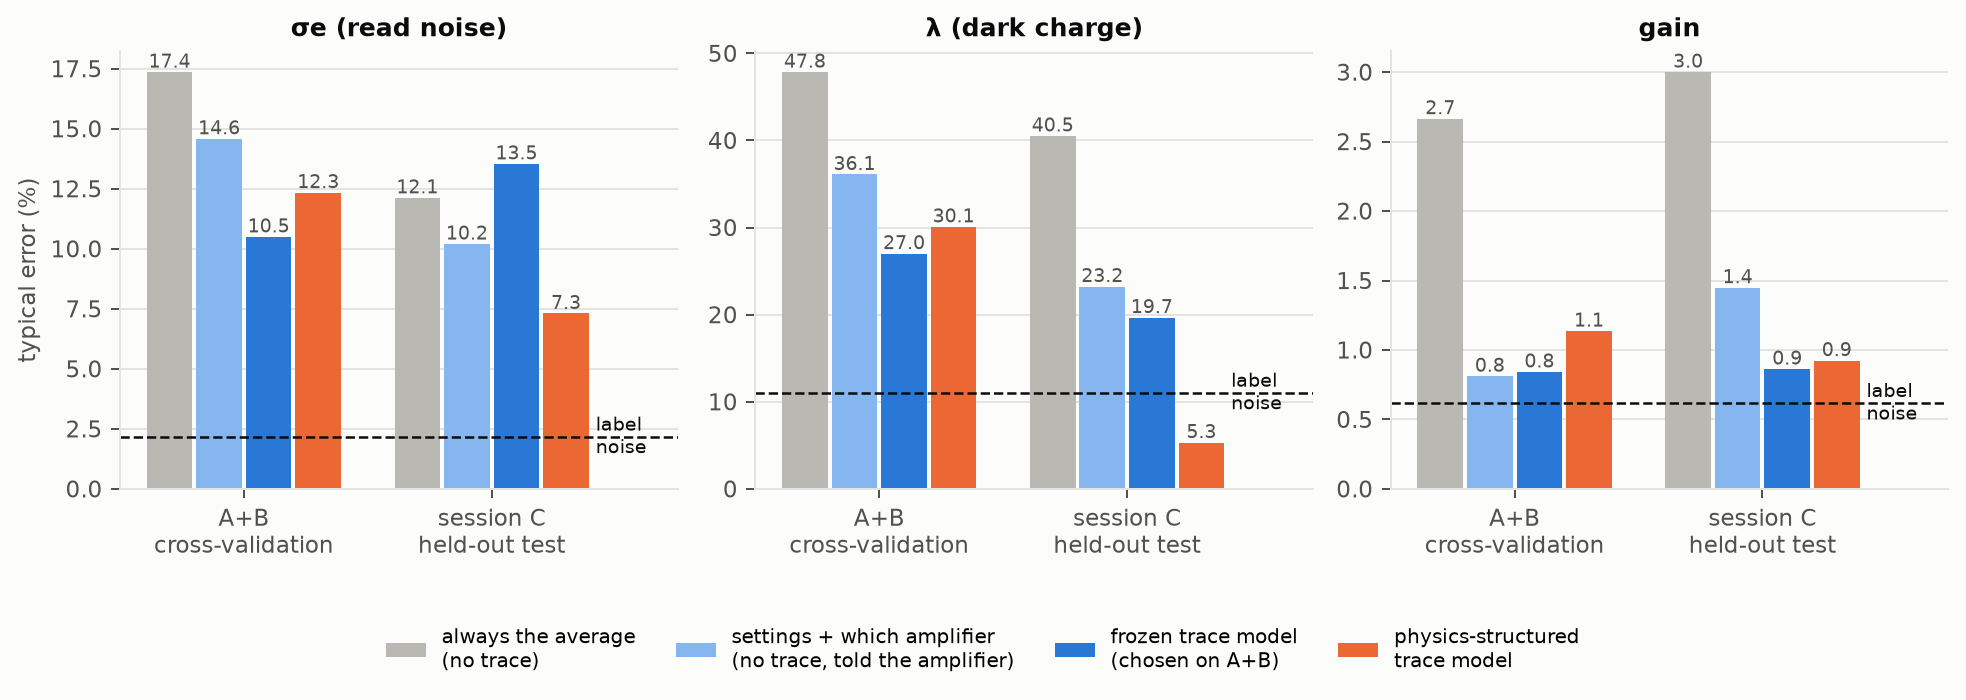
\includegraphics[width=\textwidth]{figures/fd_fig1_traces_help.png}
\caption{Typical error of the average, settings + amplifier name (no trace), the model frozen on A+B and the
physics-structured model, on A+B cross-validation and session C. Dashed: label scatter.}
\label{fig:help}
\end{figure}

On session C the physics model predicts $\lambda$ to 5.3\,\% (23.2\,\% without a trace, significant), $\sigma_e$ to
7.3\,\% (10.2\,\%) and the gain to 0.9\,\% (1.4\,\%). The model frozen on A+B failed for $\sigma_e$: A+B changes one knob
at a time, so its cross-validation tested extrapolation and rewarded flexible models; session C tests interpolation.

\begin{figure}[h]
\centering
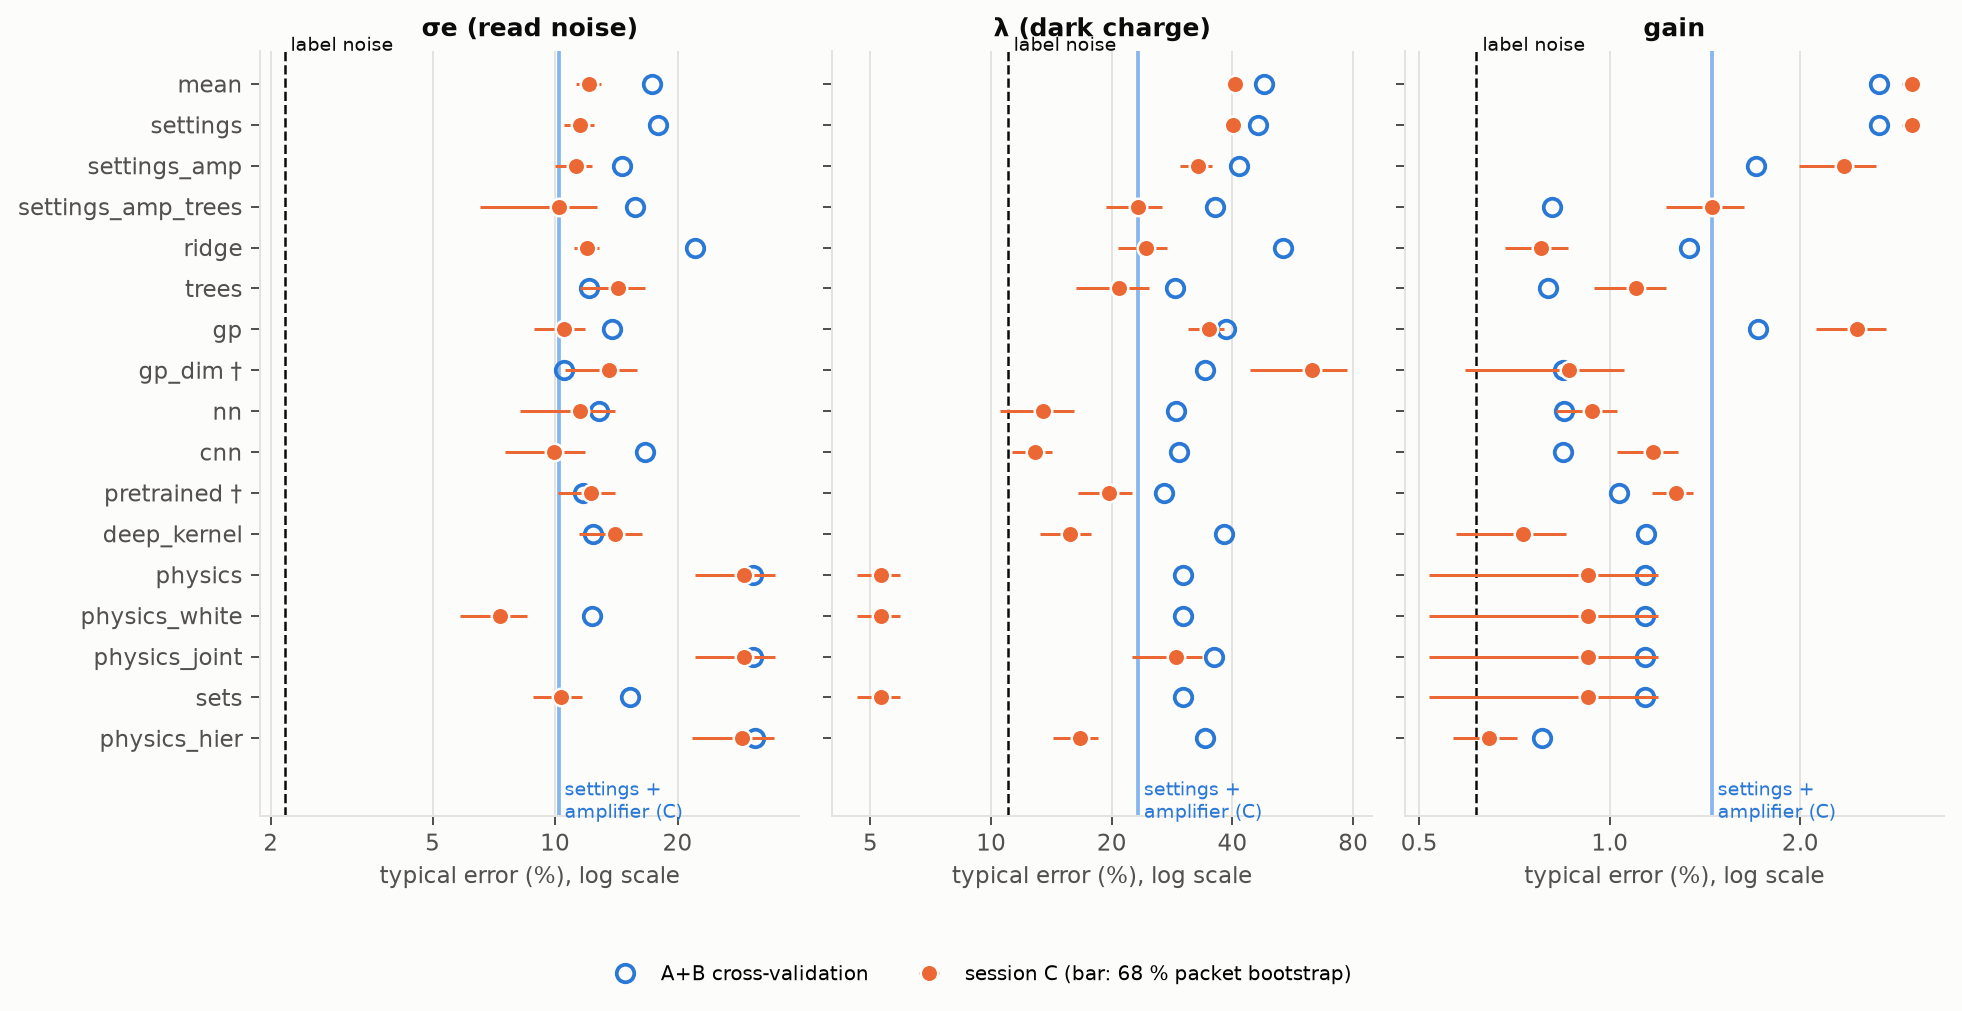
\includegraphics[width=0.9\textwidth]{figures/fd_fig7_all_models.png}
\caption{Every model: A+B cross-validation (open) and session C (filled, 68\,\% bootstrap interval).}
\end{figure}

\textbf{Where the errors come from.} Session A (timing) is 43\,\% of the rows but 76\,\% of the squared $\sigma_e$
error: timing changes move the image's noise in ways the 10-pixel trace does not see (the image reads $10^4$ pixels
after a 5300-column prescan and a register clear). $\lambda$ drifted down about 20\,\% over the night at fixed settings,
and L1\_18 waited 38 minutes without a flush before its image.

\begin{figure}[h]
\centering
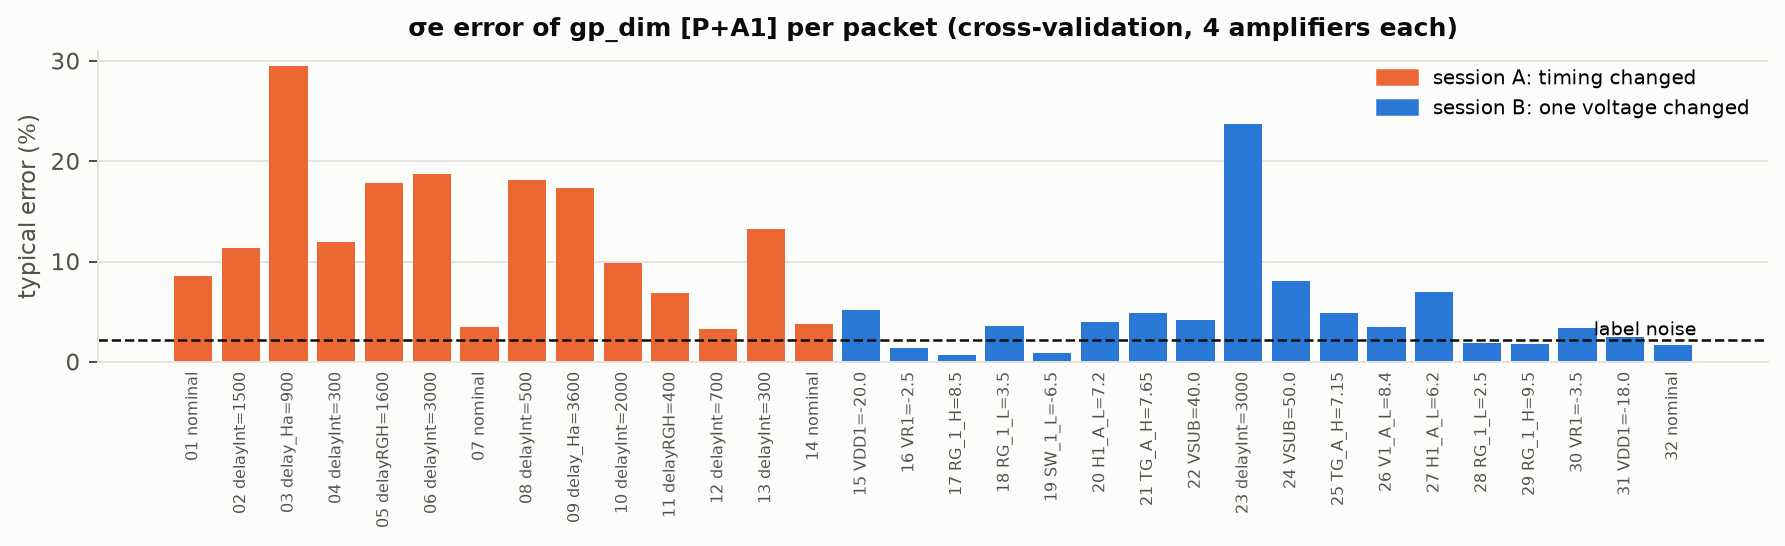
\includegraphics[width=0.49\textwidth]{figures/fd_fig3_sigma_error_by_packet.png}\hfill
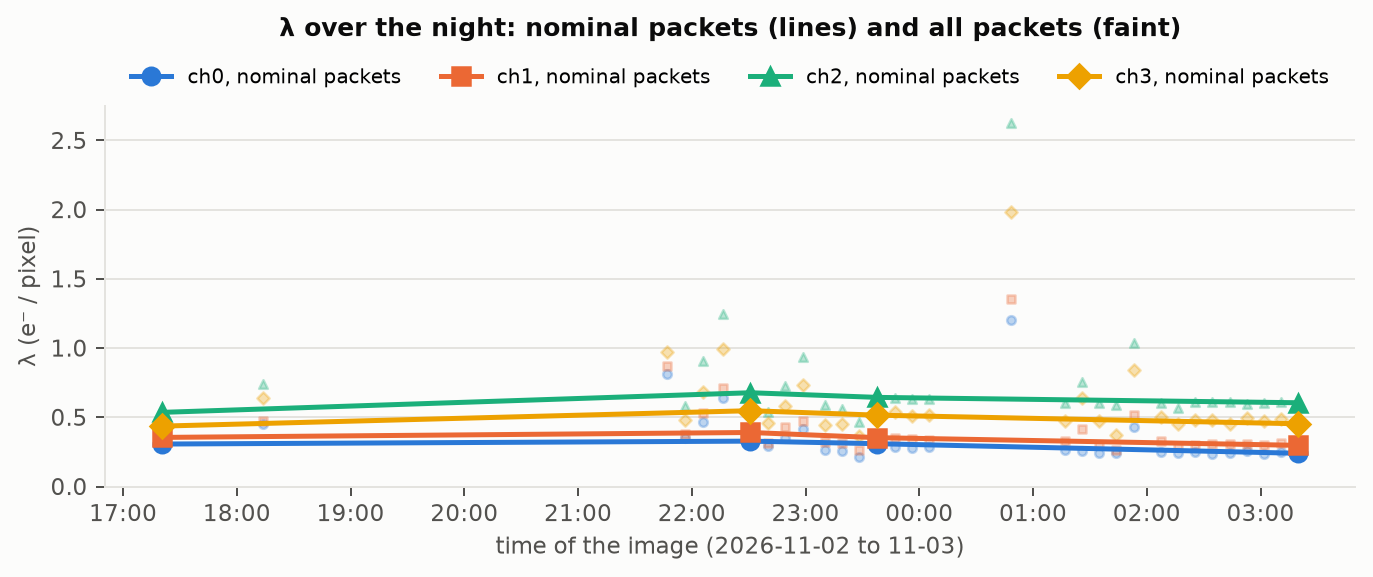
\includegraphics[width=0.49\textwidth]{figures/fd_fig5_lambda_night.png}
\caption{Left: $\sigma_e$ error per A+B packet (timing packets largest). Right: $\lambda$ of the nominal packets over
the night.}
\end{figure}

% ======================================================================================================
\section{What the models learned (2026-11-04)}

\subsection{What each model relies on}
Each model was fitted once on A+B and one group of inputs at a time was shuffled between rows (no refit):
\begin{equation}
S_G=100\sqrt{\tfrac1n\textstyle\sum_i\big(\hat y_i^{(\pi_G)}-\hat y_i\big)^2}\ \%,\qquad L_G=\mathrm{err}_C^{(\pi_G)}-\mathrm{err}_C .
\end{equation}
$S_G$ is what the model uses, $L_G$ what helps on new packets. Shuffling only within each amplifier removes ``which
amplifier this is''.

\begin{figure}[h]
\centering
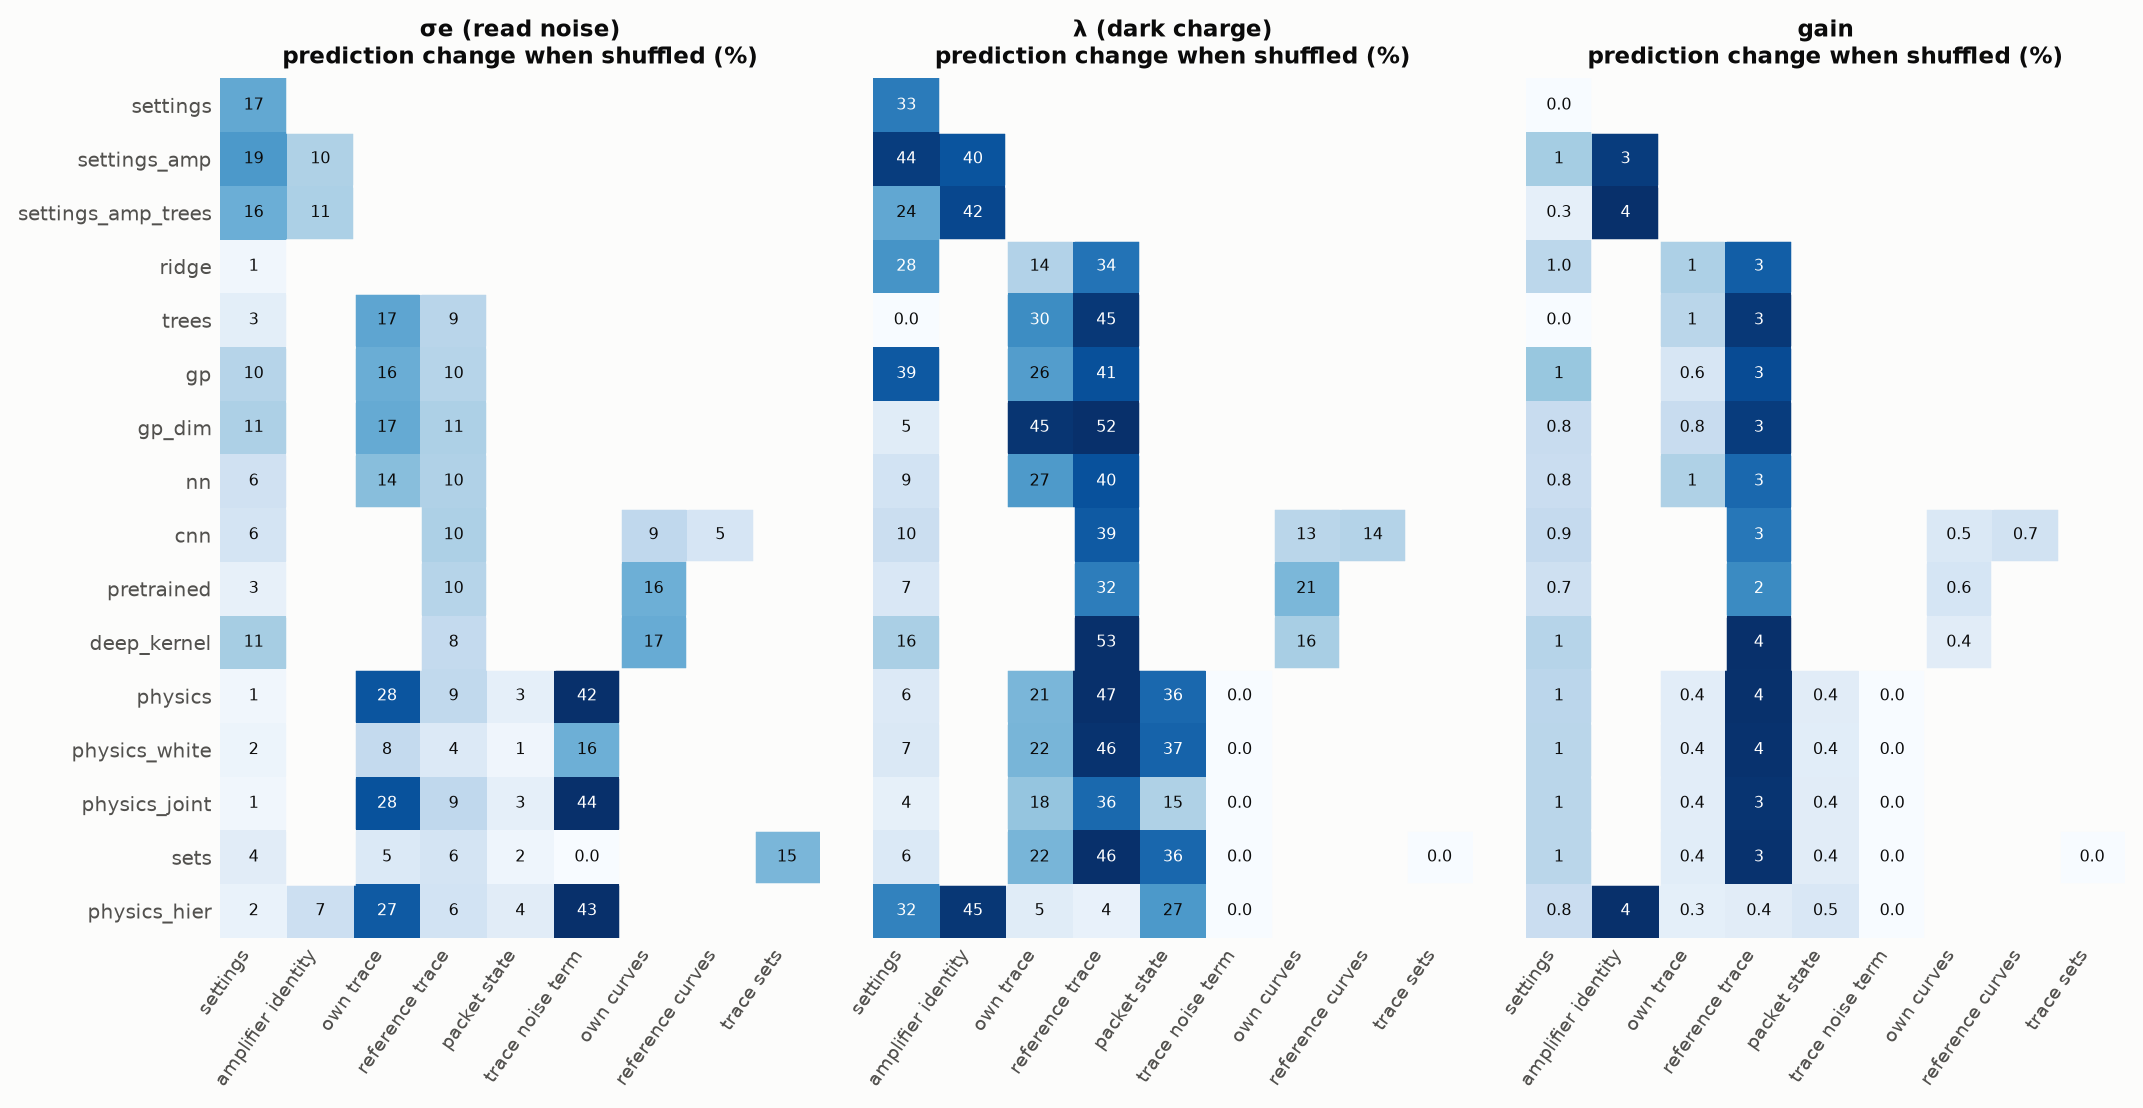
\includegraphics[width=0.85\textwidth]{figures/fd_fig8_reliance.png}
\caption{How far each model's prediction moves when an input group is shuffled.}
\end{figure}

\begin{figure}[h]
\centering
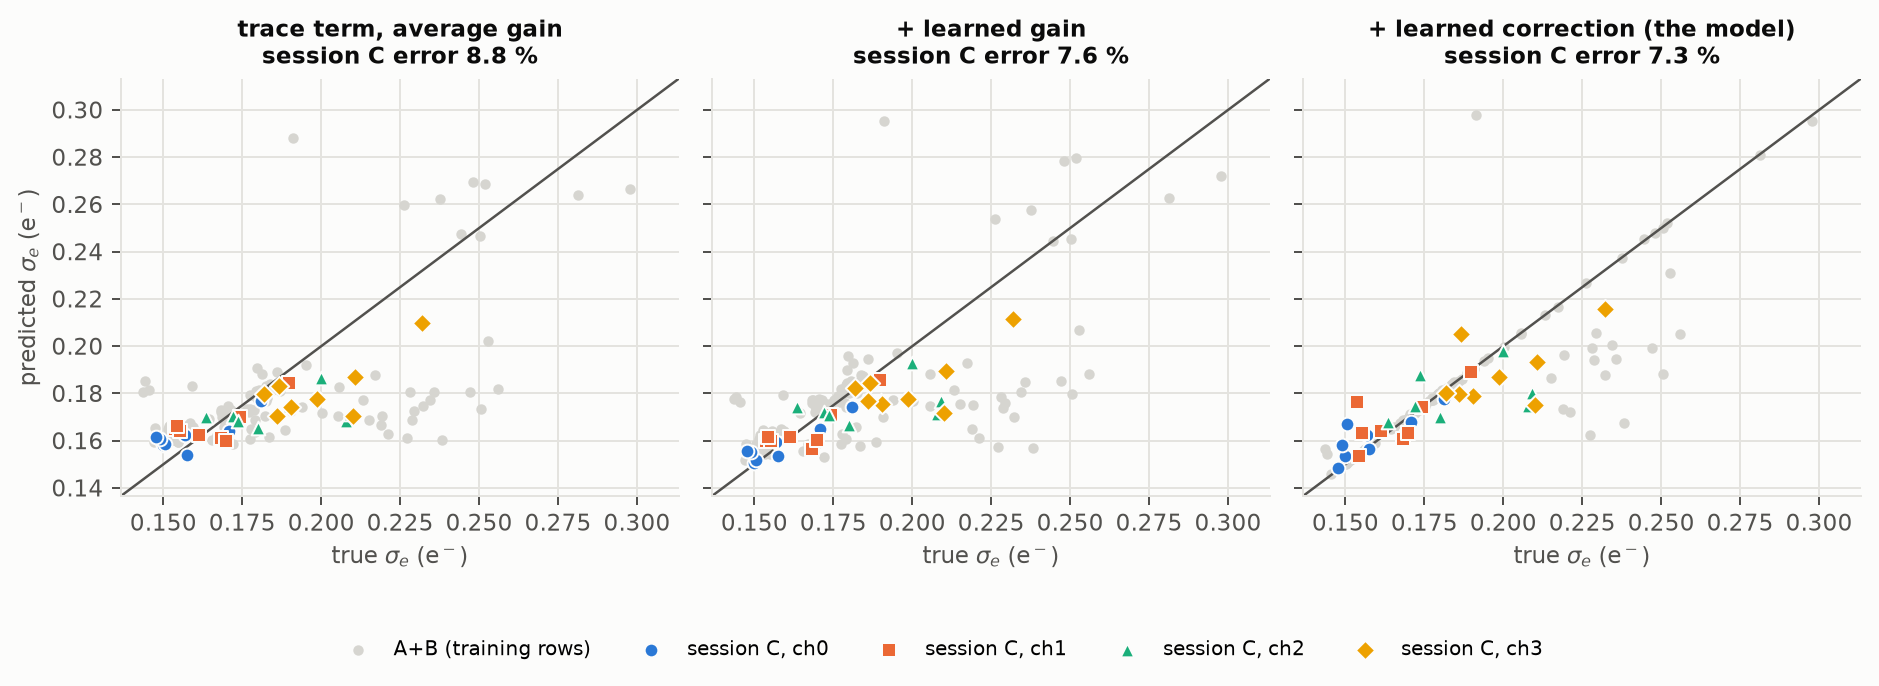
\includegraphics[width=0.9\textwidth]{figures/fd_fig9_physics_terms.png}
\caption{The physics $\sigma_e$ term by term on session C: trace term with the average gain 8.8\,\%, with the learned
gain 7.6\,\%, with the correction 7.3\,\% (the image's noise is about $0.82\times$ the trace's).}
\end{figure}

\subsection{Amplifier fingerprints}
With $\eta^2=1-\sum_a\sum_{i\in a}(x_i-\bar x_a)^2/\sum_i(x_i-\bar x)^2$ the share of a feature's variance that is
just ``which amplifier'', 52 feature columns have $\eta^2>0.9$ (46 of them reference-trace features, taken at nominal,
so only the amplifier and slow drift change them). The own trace's noise features are not fingerprints (white noise:
$\eta^2=0.09$). The gain and $\lambda$ predictions leaned on these fingerprints.

\begin{figure}[h]
\centering
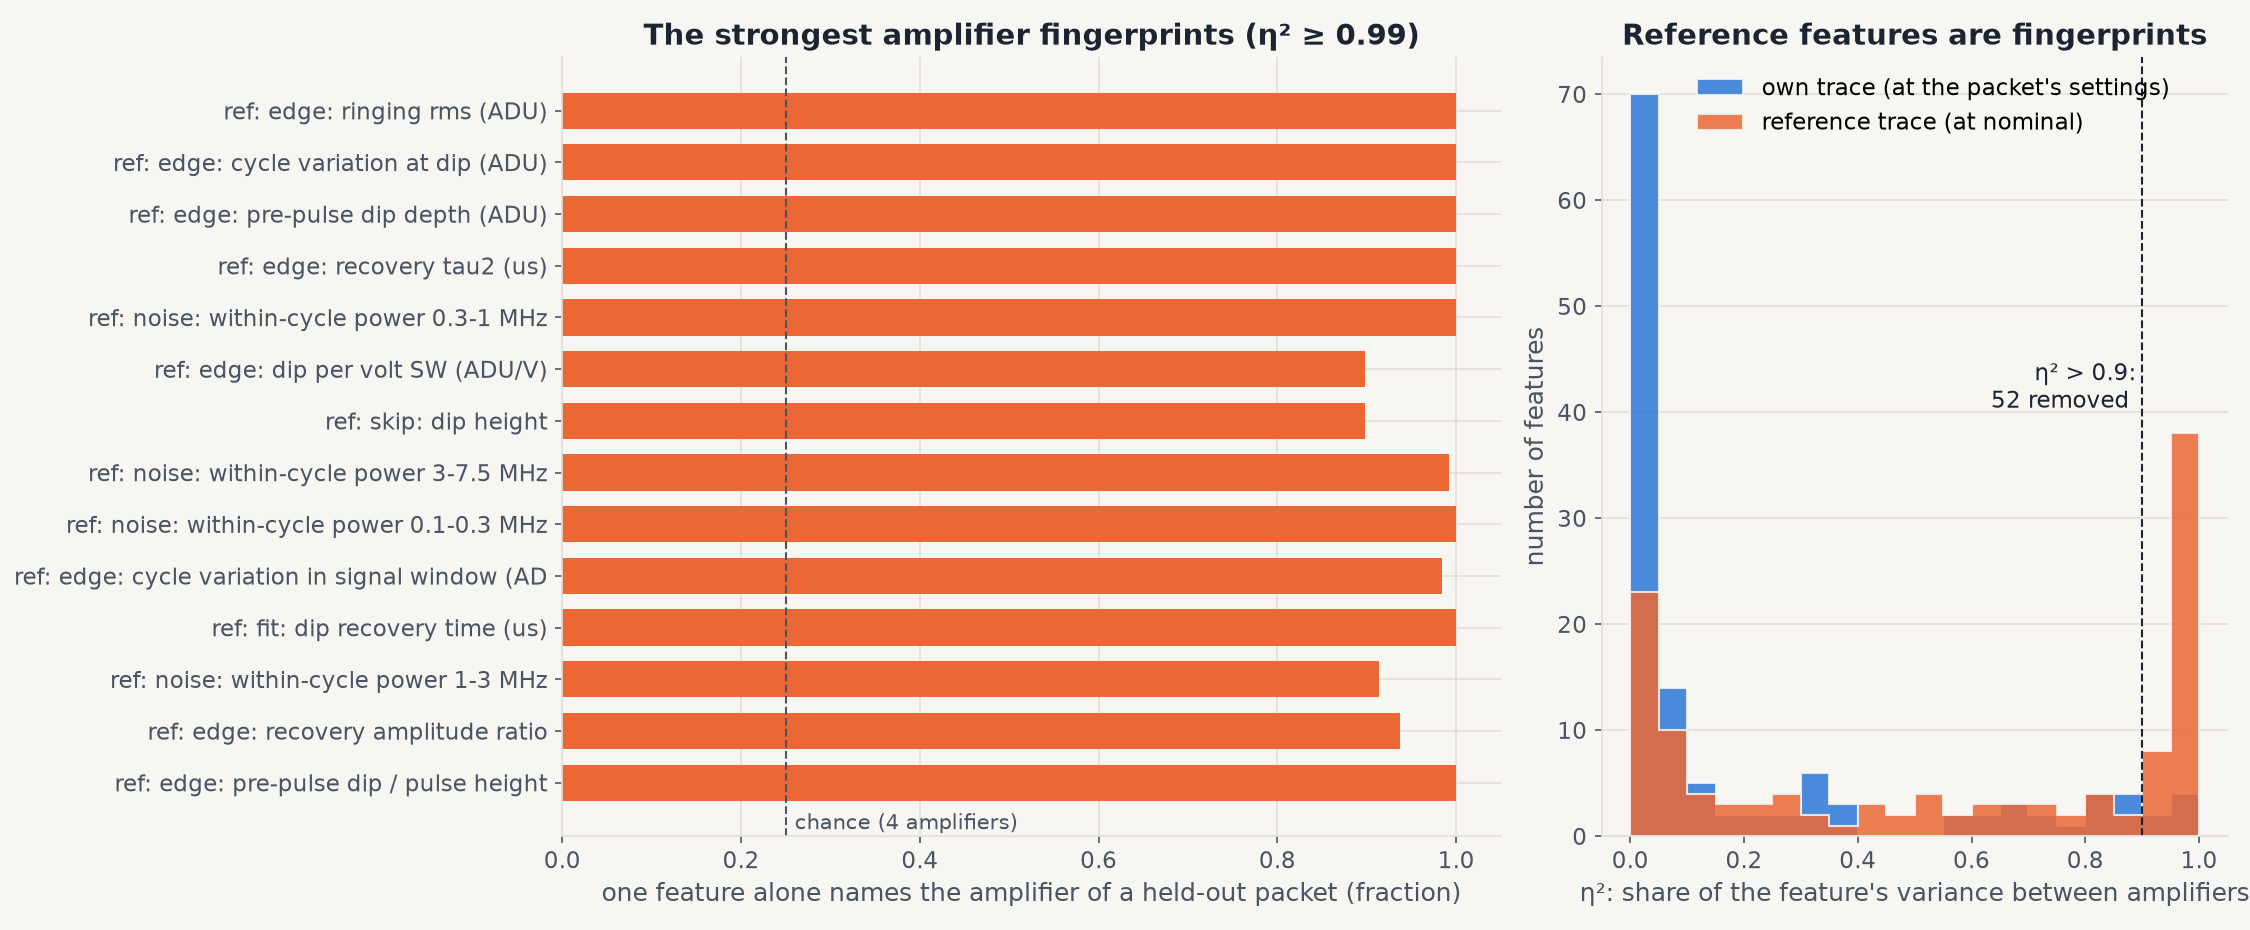
\includegraphics[width=0.85\textwidth]{figures/fig_fingerprint.png}
\caption{Left: features that alone name the amplifier of a held-out packet. Right: $\eta^2$ of own and reference
features.}
\end{figure}

\subsection{New amplifiers}
Leave one amplifier out (train on three, predict the fourth, crossed with the packet folds): only the $\sigma_e$
physics model beats the average on an unseen amplifier (14.0\,\% against 18.7\,\%). For $\lambda$ and the gain no model
beats the average until the amplifier's offset is removed (``after one image''); then the gain is at about 1\,\%.

\begin{figure}[h]
\centering
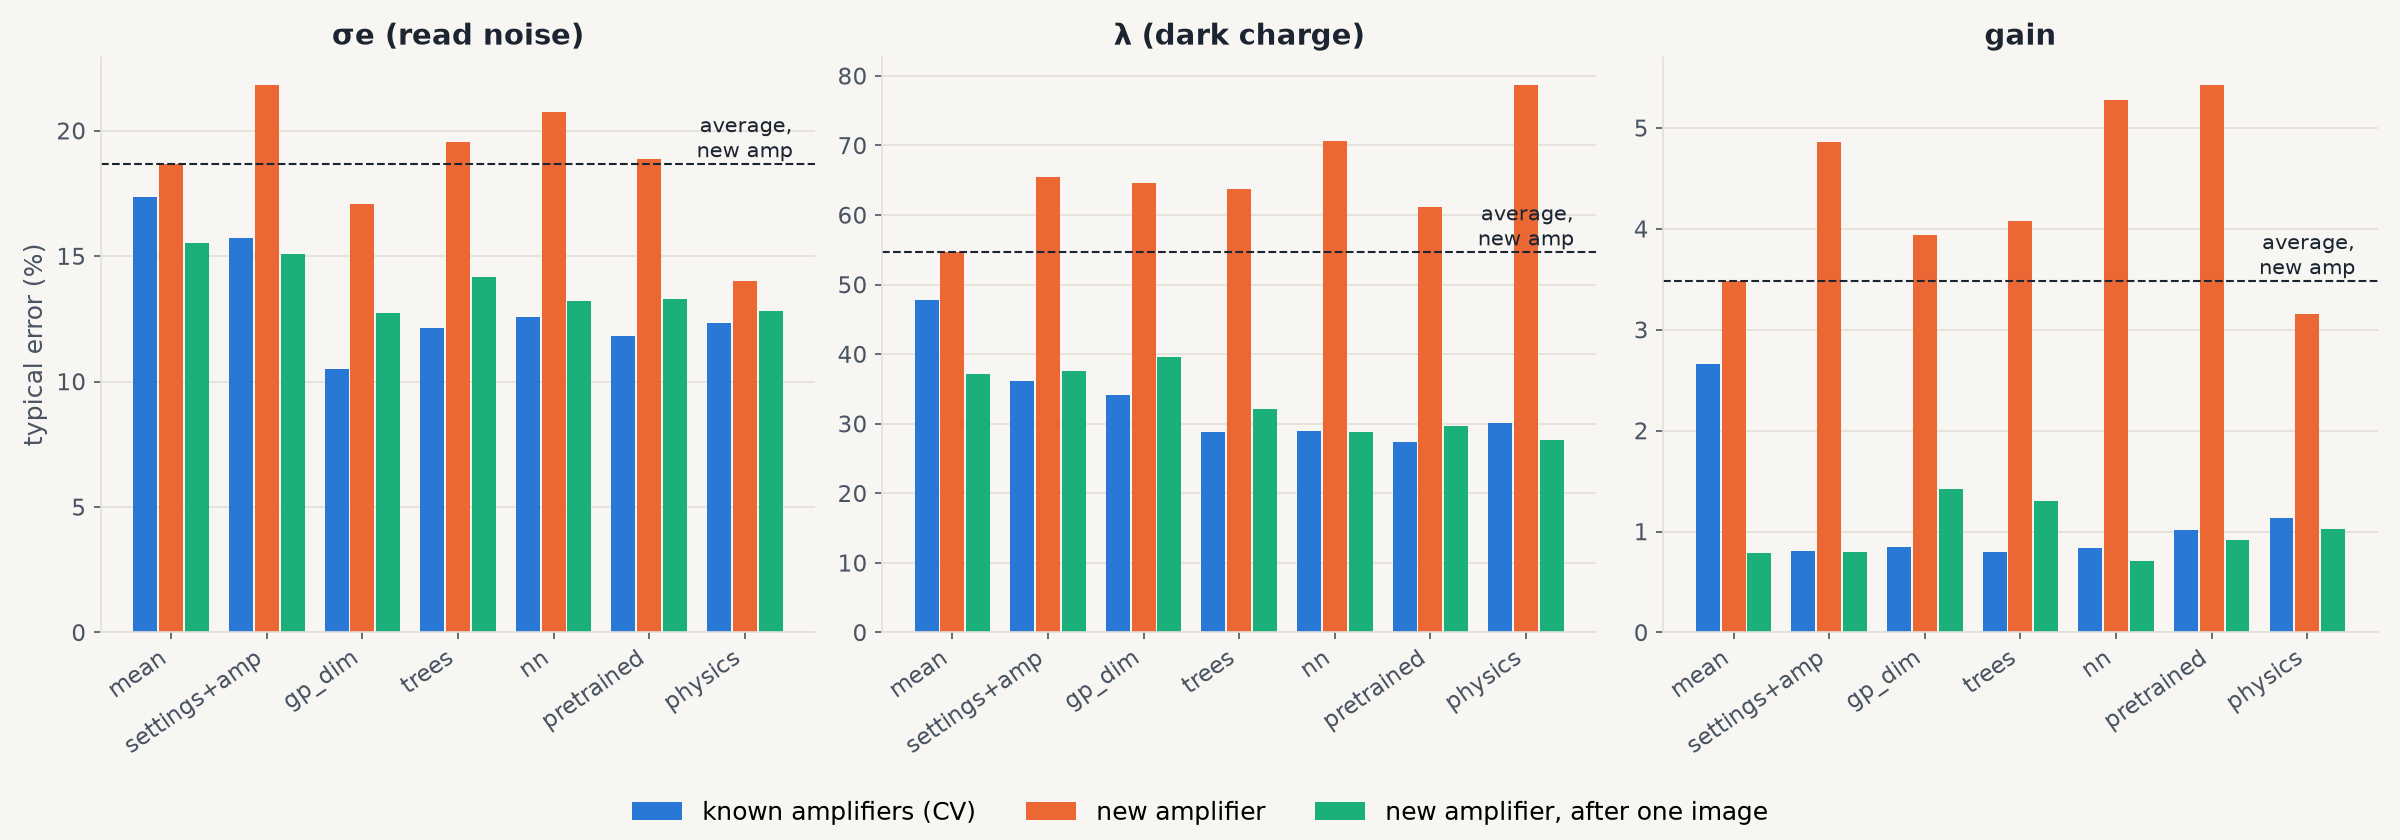
\includegraphics[width=\textwidth]{figures/fig_loao.png}
\caption{Error on known amplifiers, on a new amplifier, and on a new amplifier after one calibration image.}
\end{figure}

\textbf{Why recognising the amplifier is not predicting its gain.} On known amplifiers a model learns a lookup
(fingerprint $\to$ amplifier $\to$ its gain). A new amplifier's fingerprint has no gain attached, and three training
amplifiers are three points. Physically, the trace is in ADU and holds no known charge: $\sigma_1^{\rm ADU}=\sigma_e
g$, so a quiet high-gain amplifier looks like a noisy low-gain one. Only whole electrons (the image's or a strip's
peaks) separate them.

\textbf{Board 102.} Trained on board 101 and tested on board 102 ch2 (102 sat at nominal all night; ch0 and ch1 are
dead): the $\sigma_e$ level is about 30\,\% off (image/trace ratio 1.06 on 102 against 0.82 on 101) and $\lambda$
(1.11, 2--4$\times$ board 101) about 90\,\% off; after one image every model is at the label scatter.

\subsection{Without the noisy channel, the fingerprints and the settings}
Board 101 ch2 (EXT3) has a per-row fit $\chi^2$ of 22 (others 3--4) and $\lambda=0.61$ (others 0.27--0.48). Table
\ref{tab:clean} compares training choices, always scored on ch0, ch1 and ch3.

\begin{table}[h]
\centering\small
\begin{tabular}{llcccc}\toprule
target & model & with ch2 & no ch2 & + no fingerprints & + no settings\\\midrule
\multicolumn{6}{l}{\textit{session C (known amplifiers)}}\\
$\sigma_e$ & physics & 6.7 & 6.2 & 5.9 & 6.1\\
$\lambda$ & physics & 5.3 & 7.0 & 10.4 & 10.4\\
$\lambda$ & cnn & 14.0 & 12.5 & 13.2 & 11.8\\
gain & physics & 1.0 & 0.7 & 2.0 & 0.7\\
\multicolumn{6}{l}{\textit{new amplifier}}\\
$\sigma_e$ & physics & 14.4 & 14.8 & 14.4 & 14.9\\
$\lambda$ & physics & 70.0 & 48.9 & 46.3 & 46.0\\
$\lambda$ & cnn & 47.8 & 49.0 & 44.4 & 39.7\\
$\lambda$ & average & 52.0 & 51.5 & 51.5 & --\\
gain & physics & 2.9 & 3.6 & 3.6 & 3.7\\\bottomrule
\end{tabular}
\caption{Errors (\%) on ch0, ch1, ch3. Each column also includes the changes to its left.}
\label{tab:clean}
\end{table}

Leaving out ch2 lets the $\lambda$ models beat the average on a new amplifier; removing the fingerprints costs
$\lambda$ on known amplifiers but not on new ones; removing the settings costs nothing. The models therefore learn from
the trace, not from a map of this CCD's knobs.

\subsection{Learning curve}
Trained on random subsets of A+B (without ch2 and the fingerprints) and scored on session C, $\sigma_e$ (physics)
falls from 9.7\,\% to 5.9\,\% and $\lambda$ from 19.0\,\% to 10.4\,\% between 8 and 32 packets, still falling; the gain
levels off near 1\,\%.

\begin{figure}[h]
\centering
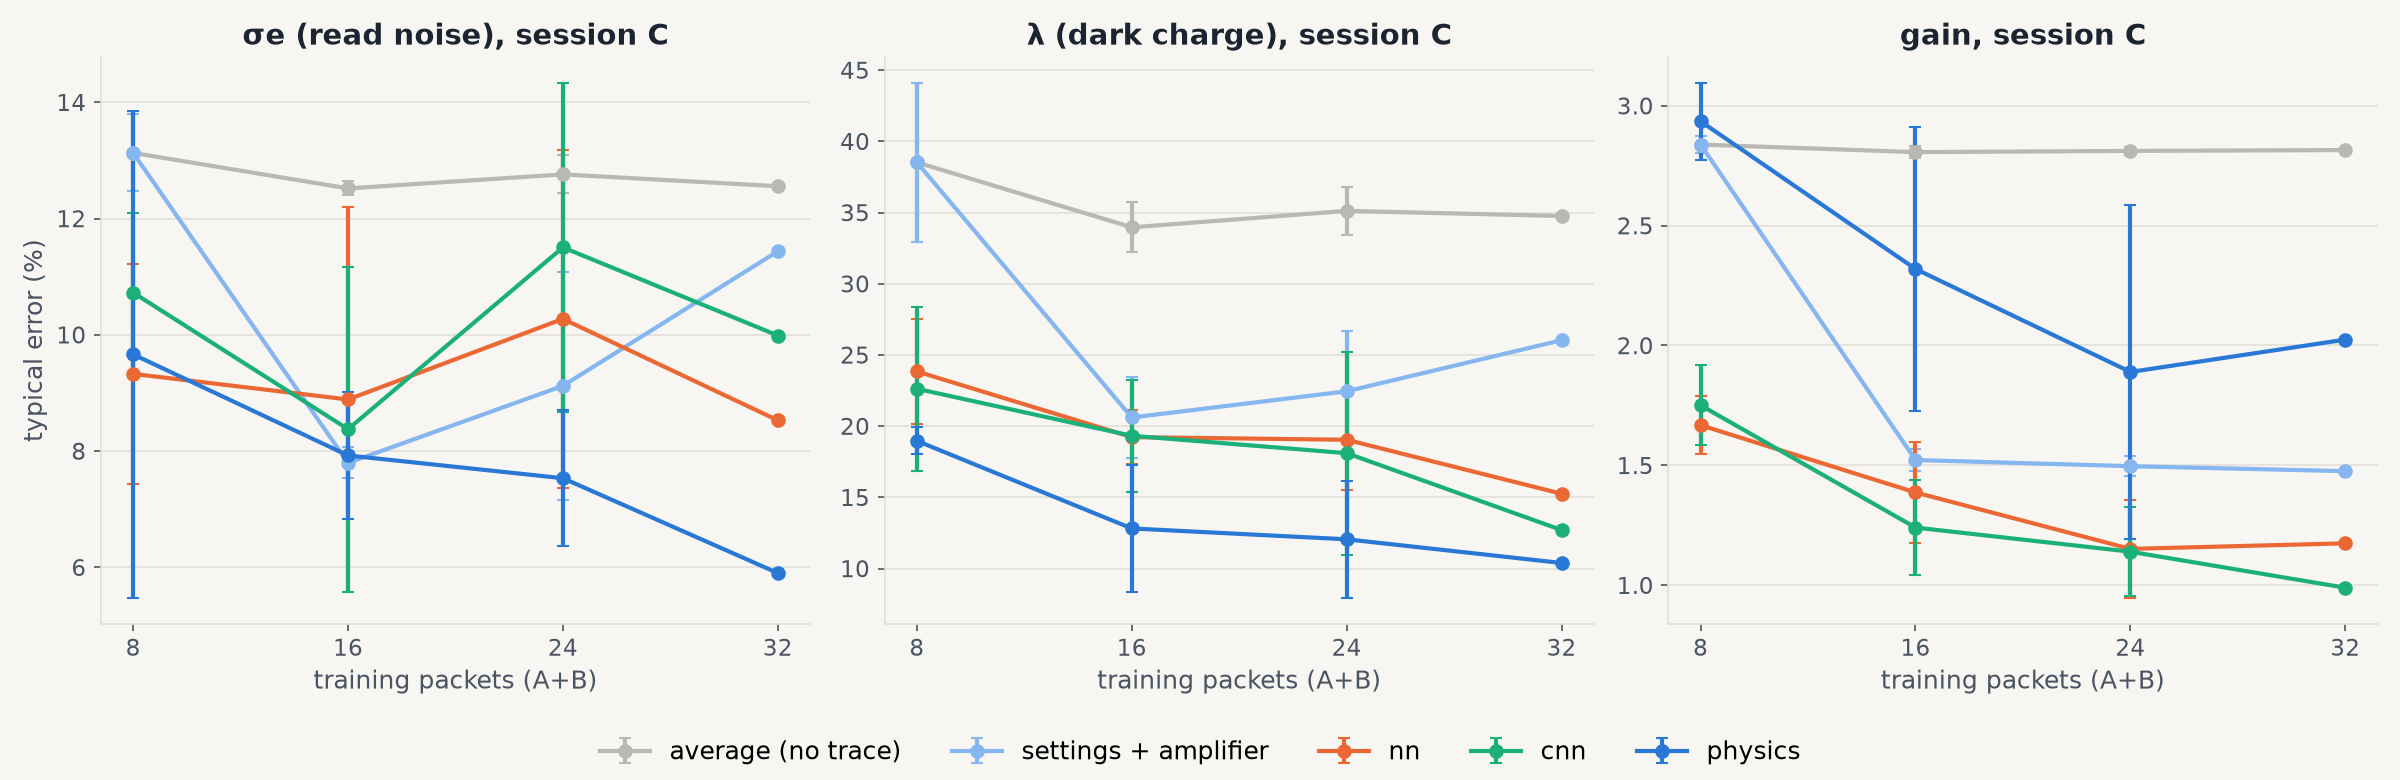
\includegraphics[width=\textwidth]{figures/fig_learning_curve.png}
\caption{Session C error against the number of training packets (5 random draws per size).}
\end{figure}

% ======================================================================================================
\section{What carries over to another CCD}

\begin{equation}
\log y(\theta,a)=c_a+f(\theta,\text{trace}),\qquad c_a=\log y_{\rm measured}(\theta_0)-f(\theta_0).
\end{equation}
The model $f$ learns how each quantity changes with the settings and the CCD's state; $c_a$ is one number per amplifier
and target, measured once from an image or a level-1 strip at nominal. The gain and the $\sigma_e$ factor are stable
(0.6\,\%, 2\,\% over a night); $\lambda$ drifts and needs re-anchoring. The ideal model takes a trace at the settings to
try plus the per-amplifier calibration and returns $\sigma_e$, $\lambda$ and $g$ with error bars, at the cost of a
trace instead of an image.

% ======================================================================================================
\section{Next steps}

\textbf{Level-1 strips.} A $2\times1000$-pixel strip with 500 skips, read after the same prescan and clear as the image
(src/decode\_l1.py, src/l1\_features.py), gives each amplifier's gain from the peak spacing (about 1\,\%), CIC plus
serial-register charge (about 5\,\%, most of $\lambda$ on board 101) and $\sigma_e$; true dark current only weakly,
since strip rows barely wait. Every model will be scored on traces, strips and both, on the same rows.

\textbf{The v2 packets.} Reset and readback, flush, 3 reference trace sets (checked), reference strip, flush, change,
2 settle traces, 5 new sets (checked), new strip, flush, a 32-row image, flush and reset. 76 packets (61 training in a
joint Sobol design over 12 knob groups, nominal every 7, 3 replicates; 15 held out), about 21 hours.

\begin{enumerate}
\item Before the v2 night: the DAQ strip test ($1\times500$, $1\times1000$, $2\times1000$), pull main on the DAQ
  machine, change settings on every working board.
\item After v2: traces vs strip vs both; train without ch2, fingerprints and settings; choose on joint data, freeze,
  score session E once.
\item Later: train on one CCD and test on another; a $\lambda$ formula (dark current $\times$ wait time + CIC); level 2,
  safe Bayesian optimisation of the settings.
\end{enumerate}

\end{document}
